% =====================================================================
%  GMN2 §7.5–7.8  从三角剖分到 KS 辛同胚 / 特殊 ϑ 处的跳变 / 二次加细 / 关于全谱的评论
%  原文：wkb-paper.tex 5419–5954 行；印刷页 p.90–99
%  编号公式 (7.23)–(7.68) 共 46 条（已对照原文 PDF 逐段核过首末号）
%  脚注 2 条；插图 6 幅：图 36 flip-cycles、37 anti-cells、38/39 wkb-m±1（原文
%  \instwofigs 并排、两个 \caption，占两个图号）、40 limit-homology-annulus、
%  41 degenerate-combining-loops；另引用第 6 节的图 28（spiral-jump）
%  ch10 自 5419 行起，含 §7.5 正文（ch09 止于 5418）
%  块内公式用 \eqref；跨块引用硬编码原文编号并加 % TODO 合稿改 \ref / \eqref
% =====================================================================

\subsection{从三角剖分到 KS 辛同胚}

我们简短地盘点一下目前的进展。我们刚刚从 WKB 分析看到：坐标系 $\CX^{T_\WKB}$ 的渐近性质，可以用相应装饰三角剖分 $T_\WKB$ 的某些简单性质很好地刻画。对 $\zeta$-平面中绕原点的任意一个张角不超过 $\pi$ 的扇形 $\CV$，都可以联系一个由装饰三角剖分构成的、性状良好的子群胚 $\CT_\CV$。一个三角剖分属于 $\CT_\CV$，是指可以为其各边选取同伦代表，使之具有两条基本性质：a) 对一切 $\zeta\in\CV$，沿各边走向奇点时装饰是指数式小的；b) 沿每条边，$\lambda\cdot\partial_t$ 落在 $\CV$ 中（对 $\lambda$ 的符号作某种选取）。WKB 分析告诉我们：第 5 节% TODO 合稿改 \ref{sec:fg-coordinates}
中定义的函子，把 $\CT_\CV$ 中每个三角剖分映为扇形 $\CV$ 内具有「良好渐近」的一个达布坐标系。所谓良好渐近，指的是：每个函数都自然地用一个 $\hat\Gamma$ 中的圈来标记，并且当 $\zeta\in\CV$ 时，$\lim_{\zeta\to0}\CX_\gamma(\zeta)\exp\left[-\zeta^{-1}\pi R Z_\gamma\right]$ 有限。

由于这种标记，我们可以把每个坐标系都看作到某个抽象复环面的映射，该环面带一组傅里叶模 $\CX_\gamma$；而每个坐标变换就简单地是那个环面的一个辛同胚。对任意满足 $\vartheta_+-\vartheta_-\le\pi$ 的 $\vartheta_+,\vartheta_-$，联系坐标系 $\CX^{\vartheta_\pm}_\gamma$ 的坐标变换是一个有意思的辛同胚 $\mathbf{S}(\vartheta_+,\vartheta_-;u)$。为预先照顾到后面的结果，我们沿用第 2 节% TODO 合稿改 \ref{sec:review}
的命名。按构造，若 $\vartheta_-<\vartheta<\vartheta_+$，则 $\mathbf{S}(\vartheta_+,\vartheta_-;u)=\mathbf{S}(\vartheta_+,\vartheta;u)\,\mathbf{S}(\vartheta,\vartheta_-;u)$。

第 2 节提到的「斯托克斯因子」，出现在 $\vartheta_+$ 与 $\vartheta_-$ 分别从左、右两侧趋近同一个值 $\vartheta_0=\arg Z_{-\gamma_0}$ 的极限下。此时 $\mathbf{S}(\vartheta_+,\vartheta_-;u)\to\mathbf{S}_{\vartheta_0,u}$。显然，这些斯托克斯因子由 WKB 三角剖分 $T_\WKB(\vartheta_+)$ 与 $T_\WKB(\vartheta_-)$ 之间的比较所捕获。除非三角剖分在 $\vartheta_0=\arg Z_{-\gamma_0}$ 处跳变，否则该斯托克斯因子就是恒等变换。若三角剖分确有跳变，我们就能算出相应的辛同胚。接下来几个小节就来干这件事。

根据与第 2 节的比较，我们预期——尽管在目前阶段这远非显然——$\mathbf{S}_{\vartheta_0,u}$ 只涉及由 $\CX_{\gamma_0}$ 的函数生成的辛同胚。马上就会看到，情况确实如此：$\mathbf{S}_{\vartheta_0,u}$ 是一列 KS 因子 $\CK_{n\gamma_0}$ 的乘积，其重数正是所预期的 $\Omega(n\gamma_0)$。穿墙公式在第 2 节中被写成 $\mathbf{S}(\vartheta_+,\vartheta_-;u)$ 在 $\lambda$ 作微小改变下的不变性；于是它现在直接由装饰三角剖分 $T_\WKB(\vartheta_+,\lambda^2)$ 与 $T_\WKB(\vartheta_-,\lambda^2)$ 的不变性推出。

\subsection{特殊 $\vartheta$ 处的跳变}

\subsubsection{来自 BPS 超多重态的辛同胚}

我们已经看到，当 $\vartheta$ 越过某个对应于 BPS 超多重态的临界值 $\vartheta_c$ 时，WKB 三角剖分会跳变。现在想知道 $\CX^\vartheta_\gamma$ 在这个 $\vartheta_c$ 处如何跳变。

让我们把问题陈述得稍精确一点。当 $\vartheta$ 取在小间隔 $\vartheta_-\le\vartheta<\vartheta_c$ 内时，WKB 三角剖分的同伦类不变，记作 $T_-$。类似地，考虑小间隔 $\vartheta_c<\vartheta\le\vartheta_+$ 内的 $\vartheta$，得到三角剖分 $T_+$。我们要比较 $\CX^{\vartheta_-}_\gamma$ 与 $\CX^{\vartheta_+}_\gamma$。为减轻记号负担，下文有时把 $\vartheta_\pm$ 简写成 $\pm$。

\insfig{5.75in}{flip-cycles}{联系于三角剖分 $T_\WKB(\vartheta_\pm)$ 的诸闭链。}

图 36 画出了其中一些闭链 $\gamma^\pm_E$。% TODO 合稿改 \ref{fig:flip-cycles}
从图中可以读出它们之间的关系：
%
\begin{align}
\gamma_E^{-} &= - \gamma_E^{+}, \label{eq:flip-c1} \\
\gamma_{E_{12}}^{-} &= \gamma_{E_{12}}^{+}, \label{eq:flip-c2} \\
\gamma_{E_{41}}^{-} &= \gamma_{E_{41}}^{+} - \gamma_E^{-}. \label{eq:flip-c3}
\end{align}
%
最后两式可以简洁地概括为变换
$\gamma_{E_i}^+ = \gamma_{E_i}^- + \inprod{\gamma_{E_i}^-, \gamma_E^-}_{{}_+} \gamma_E^-$，
其中交积上的下标 $+$ 表示只取正的部分。

现在可以描述 flip 前后 $\CX_\gamma$ 之间的关系了。首先，由 (5.15)% TODO 合稿改 \eqref{eq:fg-trans-1}
看到
\begin{equation}
\CX^+_E = 1/\CX^-_E.
\end{equation}
把它与 \eqref{eq:flip-c1} 结合，并随意使用由诸 $\CX_E$ 定义 $\CX_\gamma$ 的定义式，得到
\begin{equation}
\CX^+_{\gamma_E^+} = (\CX^-_{\gamma_E^-})^{-1} = \CX^-_{\gamma_E^+}.
\end{equation}
换句话说，$\CX_{\gamma_E^+}$ 跨越射线 $\vartheta=\vartheta_c$ 时是连续的。

接下来考虑边 $E_{12}$。由 (5.16)% TODO 合稿改 \eqref{eq:fg-trans-2}
有
\begin{equation}
\CX^+_{E_{12}} = \CX^-_{E_{12}} (1 + \CX^-_E).
\end{equation}
把它与 \eqref{eq:flip-c2} 结合，得到
\begin{equation}
\CX^+_{\gamma^+_{E_{12}}} = \CX^-_{\gamma^+_{E_{12}}} (1 + \CX^-_{\gamma^-_E}).
\end{equation}
对 $\CX^\pm_{\gamma_{E_{34}}}$ 有同样的结论，只须把上式中的 $1\to3$、$2\to4$。

$E_{41}$ 的故事稍复杂些。由 (5.19)% TODO 合稿改 \eqref{eq:fg-trans-5}
有
\begin{equation}
\CX^+_{E_{41}} = \CX^-_{E_{41}} (1 + (\CX^-_E)^{-1})^{-1}.
\end{equation}
把它与 \eqref{eq:flip-c3} 结合，得到
\begin{equation}
\begin{split}
\CX^+_{\gamma^+_{E_{41}}} &= \CX^-_{\gamma^-_{E_{41}}} (1 + (\CX^-_E)^{-1})^{-1}
= \CX^-_{\gamma^+_{E_{41}}} (\CX^-_E)^{-1} (1 + (\CX^-_E)^{-1})^{-1} \\
&= \CX^-_{\gamma^+_{E_{41}}} (1 + \CX^-_E)^{-1}.
\end{split}
\end{equation}
对 $\CX^\pm_{\gamma_{E_{23}}}$ 有同样的结论，只须把上式中的 $4\to2$、$1\to3$。

为总结所得结果，我们定义
\begin{equation}
\gamma_{\rm hyper} := \gamma^-_E.
\end{equation}
这就是由那条有限 WKB 曲线所代表的 BPS 超多重态的电荷。我们得到的是
\begin{equation} \label{eq:KS-flip}
\CX^+_\gamma = \CX^-_\gamma (1 + \CX^-_{\gamma_{\rm hyper}})^{\inprod{\gamma, \gamma_{\rm hyper}}}.
\end{equation}
若取 $\Omega(\gamma_{\rm hyper})=1$——这与「该有限 WKB 曲线代表一个电荷为 $\gamma_{\rm hyper}$ 的单个 BPS 超多重态」恰好相符——并取 $\sigma(\gamma_{\rm hyper})=-1$、且对所有 $n>1$ 取 $\Omega(n\gamma_{\rm hyper})=0$，那么这正是所预期的变换性质 (2.7)。% TODO 合稿改 \eqref{eq:ks-discontinuity}

\subsubsection{来自 BPS 矢量多重态的辛同胚}

现在考虑 $\vartheta_c$ 对应于矢量多重态时会发生什么。此时，如第 6.6.3 节% TODO 合稿改 \ref{sec:vector-jump}
所讨论，$\vartheta_c$ 附近的 WKB 三角剖分含一个环带 $W$，而构成 $W$ 之三角剖分的那些边，在从任一侧令 $\vartheta\to\vartheta_c$ 时都经历一列无穷多次 flip；恰在 $\vartheta_c$ 处，我们有一个被闭合 WKB 曲线叶层化的环带。

下文将用到关于 WKB 叶层化的一些论断，它们是由计算机实验确定的。我们相信，所描述的图景至少在 $C$ 亏格为零时是正确的；不过，在本文第一个预印本版本出现之后，Ivan Smith 向我们指出：若 $C$ 的亏格 $g>0$，且环带 $W$ 截出一个含把手、不含穿刺点的连通分支，则图景可能更复杂。在 \cite{gmn5-to-appear}% TODO 待发表
中我们将给出研究该情形的另一种办法。我们将发现，即便在这种情形下，本分析的主要结果——下面的 \eqref{eq:twist-KS}——依然成立。

首先，为使图景固定下来，方便的做法是引入一些辅助对象，即把相位取为 $\vartheta+\frac{\pi}{2}$（而非 $\vartheta$）的 WKB 曲线；称它们为\emph{反 WKB 曲线}。一般而言，若有相位为 $\vartheta_c$ 的 BPS 态，就不会有相位为 $\vartheta_c+\frac{\pi}{2}$ 的 BPS 态；因此反 WKB 曲线在 $\vartheta=\vartheta_c$ 附近光滑地变化，而 WKB 曲线在该处正经历剧烈的变化。特别地，对 $\vartheta_c$ 两侧的 $\vartheta$，反分界线把含该环带的一个区域方便地划分成单连通胞腔。设 $\alpha$ 与 $\beta$ 是分属其中两个胞腔的两条反 WKB 曲线（如图 37 所示），% TODO 合稿改 \ref{fig:anti-cells}
而 $\hat\alpha$ 与 $\hat\beta$ 是它们到 $\Sigma$ 的提升（取反 WKB 定向）。利用这一划分，还可以对基准路径 $E_\pm$ 作一个典范的选取，$E_\pm$ 也画在图 37 中。
\insfig{3.3in}{anti-cells}{环带的拓扑；绿色标出的是反 WKB 曲线，另画出两条基准路径 $E_\pm$。}

如同第 5.9 节% TODO 合稿改 \ref{sec:limit-triangulation}
，我们可以把环带的种种可能三角剖分标为 $T_m$，$m\in\IZ$。当 $\vartheta$ 从上方趋于 $\vartheta_c$ 时，WKB 三角剖分依次经过一列无穷多个三角剖分；这些三角剖分可以辨认出就是 $T_m$，其中 $m=m_+,m_++1,\dots$，$m_+$ 为某个整数。类似地，当 $\vartheta$ 从下方趋于 $\vartheta_c$ 时，WKB 三角剖分依次经过另一列三角剖分 $T_m$，其中 $m=m_-,m_--1,\dots$。于是，$m$ 充分大或充分小的那些 $T_m$ 都会作为 WKB 三角剖分出现，而 $m$ 取中间值的那些 $T_m$ 则未必。为下文记号方便，我们只看 $\vartheta$ 的一个窄区间，使 $m_+>m_-$（从而每个 $T_m$ 至多出现一次）；并对每个确实出现的 $T_m$，选一个满足 $T_\WKB(\vartheta_m)=T_m$ 的 $\vartheta_m$。

当 $m>m_+$ 时，$E_{m+}$ 从奇点 $\CP'$ 出发，从一个转向点的右侧经过，向右转，绕环带顺时针缠绕并穿过 $2m$ 条反分界线，然后在到达 $\CP$ 之前从第二个转向点附近经过。$E_{m-}$ 类似，但只穿过 $2m-2$ 条反分界线。$m=1$ 的情形见图 38。% TODO 合稿改 \ref{fig:wkb-m1}
\begin{figure}[htbp]
\begin{minipage}[b]{0.5\linewidth}\centering
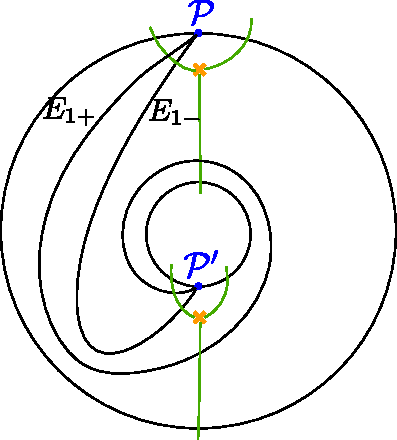
\includegraphics[width=2in]{figures/wkb-m1-crop.pdf}
\caption{$T_1=T_\WKB(\vartheta_1)$ 在环带上的拓扑。}\label{fig:wkb-m1}
\end{minipage}\hspace{0.4cm}
\begin{minipage}[b]{0.45\linewidth}\centering
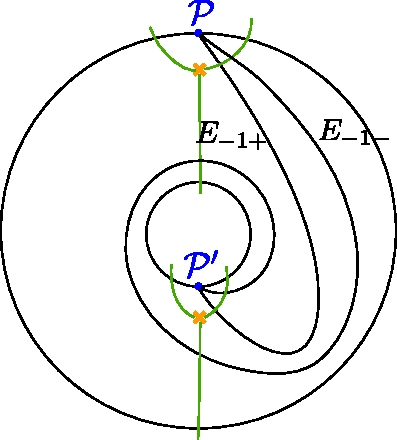
\includegraphics[width=2in]{figures/wkb-m-1-crop.pdf}
\caption{$T_{-1}=T_\WKB(\vartheta_{-1})$ 在环带上的拓扑。}\label{fig:wkb-m-1}
\end{minipage}
\end{figure}
由此可见，相应闭链满足
\begin{align}
\inprod{\gamma_{E_{m+}}^{\vartheta_m}, \hat\alpha} &= 1-m, \label{eq:int1} \\
\inprod{\gamma_{E_{m+}}^{\vartheta_m}, \hat\beta} &= 2-m, \\
\inprod{\gamma_{E_{m-}}^{\vartheta_m}, \hat\alpha} &= m, \\
\inprod{\gamma_{E_{m-}}^{\vartheta_m}, \hat\beta} &= m-1. \label{eq:int4}
\end{align}

当 $m<m_-$ 时，情况与上述非常相似，关键差别是在好几处要把「右」换成「左」。于是 $E_{m+}$ 从 $\CP'$ 出发，从一个转向点的左侧经过，向左转，绕环带逆时针缠绕并穿过 $-2m-2$ 条反分界线，然后在到达 $\CP$ 之前从第二个转向点附近经过。$E_{m-}$ 类似，但穿过 $-2m$ 条反分界线。$m=-1$ 的情形见图 39。% TODO 合稿改 \ref{fig:wkb-m-1}
此时关系 \eqref{eq:int1}–\eqref{eq:int4} 换成
\begin{align}
\inprod{\gamma_{E_{m+}}^{\vartheta_m}, \hat\alpha} &= 1+m, \label{eq:int5} \\
\inprod{\gamma_{E_{m+}}^{\vartheta_m}, \hat\beta} &= m, \\
\inprod{\gamma_{E_{m-}}^{\vartheta_m}, \hat\alpha} &= -2-m, \\
\inprod{\gamma_{E_{m-}}^{\vartheta_m}, \hat\beta} &= -1-m. \label{eq:int8}
\end{align}
现在定义四条闭链 $\gamma^\pm_{A,B}$，它们画在图 40 中。% TODO 合稿改 \ref{fig:limit-homology-annulus}
\insfig{5in}{limit-homology-annulus}{支撑在环带上方的那部分 $\hat\Gamma$ 的两组基 $\gamma^+_{A,B}$ 与 $\gamma^-_{A,B}$。}
这四条闭链满足
\begin{align}
\inprod{\gamma^+_A, \hat\alpha} = 1, \quad & \inprod{\gamma^-_A, \hat\alpha} = -1, \\
\inprod{\gamma^+_A, \hat\beta} = 1, \quad & \inprod{\gamma^-_A, \hat\beta} = -1, \\
\inprod{\gamma^+_B, \hat\alpha} = 0, \quad & \inprod{\gamma^-_B, \hat\alpha} = -2, \\
\inprod{\gamma^+_B, \hat\beta} = -1, \quad & \inprod{\gamma^-_B, \hat\beta} = -1.
\end{align}
注意由此可得
\begin{align}
\gamma^-_A &= - \gamma^+_A, \label{eq:compare-a} \\
\gamma^-_B &= - \gamma^+_B + 2 \gamma^-_A. \label{eq:compare-b}
\end{align}
另一方面，比较交积可知，这些闭链与邻近 WKB 三角剖分所附的闭链由统一公式相联系：
\begin{align}
\gamma^\pm_A & = \gamma^{\vartheta_m}_{E_{m-}} + \gamma^{\vartheta_m}_{E_{m+}}, \label{eq:gamA} \\
\gamma^\pm_B & = (1-m) \gamma^{\vartheta_m}_{E_{m-}} - m \gamma^{\vartheta_m}_{E_{m+}}, \label{eq:gamB}
\end{align}
其中左端当 $m>m_+$ 时取 $+$ 号、当 $m<m_-$ 时取 $-$ 号。

第 5.9 节中我们定义了「极限坐标系」$\CX^{T_{+\infty}}$。现在，在当前 $T_{+\infty}$ 作为 $T_\WKB(\vartheta_c)$ 出现的情形里，我们可以定义相应的同调标记：即按通常的规则 (7.3)% TODO 合稿改 \eqref{eq:canonical-darboux}
定义 $\CX^+_\gamma$，其中 $E$ 既可以指 $T_{+\infty}$ 中远离环带的一条边，也可以指特殊符号 $A$、$B$ 之一。利用 (5.32)、(5.33)、(7.48)、(7.49)，% TODO 跨块引用
可见这些坐标确实配得上「极限坐标」之名：
\begin{equation}
\lim_{\vartheta\to\vartheta_c^+} \CX^{\vartheta}_\gamma = \CX^+_\gamma. \label{eq:limit-1}
\end{equation}
类似地可以定义 $\CX^-_\gamma$；利用 (5.36)、(5.37)、(7.48)、(7.49)，% TODO 跨块引用
可见它们同样满足
\begin{equation}
\lim_{\vartheta\to\vartheta_c^-} \CX^{\vartheta}_\gamma = \CX^-_\gamma. \label{eq:limit-2}
\end{equation}

现在终于可以比较 $\CX^+_\gamma$ 与 $\CX^-_\gamma$ 了。对 $A$ 类闭链，这相当直接：利用 \eqref{eq:compare-a} 与 (5.38)% TODO 合稿改 \eqref{eq:A-relation}
可得
\begin{equation} \label{eq:twist-A}
\CX^+_{\gamma^+_A} = (\CX^-_{\gamma^-_A})^{-1} = \CX^-_{\gamma^+_A}.
\end{equation}
对 $B$ 类闭链则稍复杂些。由 \eqref{eq:compare-b} 与 (5.40)% TODO 合稿改 \eqref{eq:B-relation}
得到
\begin{equation}
\begin{split}
\CX^+_{\gamma^+_B} &= (\CX^-_{\gamma^-_B})^{-1} (\xi_+ - \xi_-)^{-4}
= \CX^-_{\gamma^+_B} (\CX^-_{\gamma^-_A})^{-2} (\xi_+ - \xi_-)^{-4} \\
&= \CX^-_{\gamma^+_B} \xi_-^{-4} (\xi_+ - \xi_-)^{-4},
\end{split}
\end{equation}
于是最终
\begin{equation} \label{eq:twist-B}
\CX^+_{\gamma^+_B} = \CX^-_{\gamma^+_B} (1 - \xi_-^2)^{-4}.
\end{equation}

定义
\begin{equation}
\gamma_{\rm vect} := - \gamma^+_A.
\end{equation}
这就是由那些闭合 WKB 曲线所代表的 BPS 矢量多重态的电荷。把结果 \eqref{eq:twist-A}、\eqref{eq:twist-B} 结合起来，得到简单的变换律
\begin{equation} \label{eq:twist-KS}
\CX^+_\gamma = \CX^-_\gamma (1 - \CX^-_{\gamma_{\rm vect}})^{-2 \inprod{\gamma, \gamma_{\rm vect}}}.
\end{equation}
注意，从图 40 可以读出 $\inprod{\gamma_B^+, \gamma_A^+}=-2$。% TODO 合稿改 \ref{fig:limit-homology-annulus}

总而言之，我们看到两个坐标系 $\CX^\pm_\gamma$ 由辛同胚 $\CK^{-2}_{\gamma_{\rm vect}}$ 相联系。于是，若取 $\Omega(\gamma_{\rm vect})=-2$——这与「闭合 WKB 曲线代表一个电荷为 $\gamma_{\rm vect}$ 的单个 BPS 矢量多重态」恰好相符——并取 $\sigma(\gamma_{\rm vect})=+1$、且对所有 $n>1$ 取 $\Omega(n\gamma_{\rm vect})=0$，我们就再次得到 $\CX_\gamma(\zeta)$ 所应满足的变换性质 (2.7)。% TODO 合稿改 \eqref{eq:ks-discontinuity}

\subsubsection{当 $m e^{-i \vartheta} \in i \IR$ 时没有辛同胚} \label{sec:no-flavor-jump}

现在处理一个棘手之处。回想每个奇点 $\CP_i$ 处都有一个参数 $m_i\in\IC$，它控制 $\varphi$ 的留数。那么，在那些使某个 $m_i e^{-i\vartheta_c}\in i\IR$ 的角度 $\vartheta=\vartheta_c$ 处，会发生什么？

如第 6.6.2 节% TODO 合稿改 \ref{sec:flavor-jump}
所述，当 $\vartheta$ 越过 $\vartheta_c$ 时，三角剖分 $T_\WKB(\vartheta)$ 在奇点 $\CP_i$ 附近跳变得相当剧烈；同时发生一次 pop，改变了平坦截面 $s_i$。另一方面，在这个 $\vartheta$ 处出现的那一族闭合 WKB 曲线并不对应带电荷的 BPS 态：它们即便是 BPS 态，也只是带味荷的态（当然，就是与穿刺点 $\CP_i$ 相关联的那个味荷）。换种说法：若按通常的办法提升这些闭合 WKB 曲线来定义 $\gamma_{\rm BPS}$，那么虽然确有 $Z(\gamma_{\rm BPS})\in e^{i\vartheta_c}\IR$，但这个电荷 $\gamma_{\rm BPS}$ 落在 $\inprod{,}$ 的根中。于是辛同胚 $\CK_{\gamma_{\rm BPS}}$ 实际上是恒等变换。因此，为与 (2.7)% TODO 合稿改 \eqref{eq:ks-discontinuity}
相容，我们应当预期：尽管 $T_\WKB$ 跳变，诸 $\CX^\vartheta_\gamma$ 在 $\vartheta=\vartheta_c$ 处\emph{不}跳变。本小节就来验证情况确实如此。

首先考虑坐标 $\CX_{C^+}$。由 (7.6)% TODO 合稿改 \eqref{eq:monodromy}
回忆到
\begin{equation}
\CX^\pm_{C^\pm} = \mu_\pm^{2}.
\end{equation}
另一方面，有
\begin{equation} \label{eq:ctrans}
C^+ = - C^-
\end{equation}
以及
\begin{equation}
\mu_+ = 1/\mu_-.
\end{equation}
于是
\begin{equation}
\CX_{C^+}^+ = (\mu_+)^{2} = (\mu_-)^{-2} = (\CX_{C^-}^-)^{-1} = \CX_{C^+}^-.
\end{equation}

\insfig{4.7in}{degenerate-combining-loops}{图 28 的一种展开；标出的是与各条边对应的同调闭链。}
还有一个 $\CX_\gamma$ 需要操心。设 $E'$ 是退化面的那条「圈」，并定义
\begin{equation}
\gamma := \gamma^{-}_{E'}.
\end{equation}
等式 $\CX^+_\gamma=\CX^-_\gamma$ 是两个不同效应相互抵消的结果。如我们在 (5.25)% TODO 合稿改 \eqref{eq:degen-loop-coord}
中所证，
\begin{equation} \label{eq:deg-1}
\CX^{\pm}_{\gamma^\pm_{E'}} = (\mu_\pm)^{-1} S,
\end{equation}
其中 $S$ 在临界迹上连续（特别地，它不涉及截面 $s$）。把图 28 展开，可以更容易看清其拓扑内容；这样得到图 41，由它可见
\begin{equation} \label{eq:degenerate-homology-jump}
\gamma^{-}_{E'} = \gamma^{+}_{E'} + C^+.
\end{equation}
把这一切合起来，即得
\begin{equation}
\begin{split}
\CX^+_{\gamma^{-}_{E'}} &= \CX^{+}_{\gamma^{+}_{E'}} \CX^{+}_{C^+} = (\mu_+)^{-1} S \mu_+^{2} \\
&= (\mu_-)^{-1} S = \CX^-_{\gamma^-_{E'}},
\end{split}
\end{equation}
正是所要的。

所以，诸 $\CX^\vartheta_\gamma$ 确实在这个 $\vartheta=\vartheta_c$ 处连续。

\subsection{二次加细} \label{sec:quadratic-refinement}

现在来看另一个烦人的细节：变换 (2.6)% TODO 合稿改 \eqref{eq:KS-Transfm}
中出现的符号 $\sigma(\gamma)$。在 \cite{Gaiotto:2008cd} 所述的一般故事中，人们预期 $\sigma:\hat\Gamma\to\IZ_2$ 是 $\hat\Gamma$ 上 mod 2 交积 $\inprod{,}$ 的一个二次加细。按定义，这意味着
\begin{equation}
\sigma(\gamma) \sigma(\gamma') = \sigma(\gamma + \gamma')\sigma(0) (-1)^{\inprod{\gamma, \gamma'}}.
\end{equation}
一般而言，人们不会指望这样的二次加细能在 $\CB$ 整体上存在；相反，必须在不同的局部补片上选取不同的加细，而在把补片粘合起来时，还必须追踪诸 $\CX^\vartheta_\gamma$ 中某些符号的变化，其来源正是这些加细彼此不同。

另一方面，在本文中我们似乎发现了一个更简单的故事。诸函数 $\CX^\vartheta_\gamma$ 的粘合律不涉及任何刁钻的符号。此外，只要取
\begin{align} \label{eq:dessigma}
\sigma(\gamma_{\rm hyper}) &= -1, \\
\sigma(\gamma_{\rm vect}) &= +1, \label{eq:dessigma2}
\end{align}
我们为诸 $\CX^\vartheta_\gamma$ 找到的变换就与 (2.6)% TODO 合稿改 \eqref{eq:KS-Transfm}
相符。这怎么能相容呢？只要存在\emph{一个}二次加细 $\sigma$，对所有在某个 $u\in\CB$ 的谱中出现的超多重态与矢量多重态都满足 \eqref{eq:dessigma}、\eqref{eq:dessigma2}，那就相容了。

对任意固定的 $(\vartheta,u)$，我们很容易构造这样的 $\sigma$：只须要求 $\sigma(0)=+1$、对 $T_\WKB(\vartheta,u)$ 的一切非退化边 $E$ 都有 $\sigma(\gamma_E)=-1$、而对退化边有 $\sigma(\gamma_E)=+1$，它就被确定了。由这个定义不难看出：对一切相位为 $\vartheta$ 的 BPS 态，都有 $\sigma(\gamma_{\rm hyper})=-1$、$\sigma(\gamma_{\rm vect})=+1$。于是从这个角度看，麻烦在于要证明如此定义的 $\sigma$ 其实与 $(\vartheta,u)$ 无关。这归结为验证：当三角剖分 $T_\WKB$ 跳变时，上述 $\sigma$ 的公式与诸 $\gamma_E$ 的变换相容。幸运的是，情况确实如此。

的确，如我们已讨论过的，随着 $(\vartheta,u)$ 变化，WKB 三角剖分经历三类变换。第一类（超多重态）由 \eqref{eq:flip-c1}–\eqref{eq:flip-c3} 给出，直接验证可知它与我们对 $\sigma$ 的提法相容。第二类（矢量多重态）用 \eqref{eq:gamA}、\eqref{eq:gamB} 所定义的辅助闭链 $\gamma_{A,B}$ 来表述；利用这两式以及我们对 $\sigma$ 的提法，可得 $\sigma(\gamma_A)=+1$、$\sigma(\gamma_B)=-1$。这个 $\sigma$ 确实与变换 \eqref{eq:compare-a}、\eqref{eq:compare-b} 相容。最后，第三类跳变（$m/e^{i\vartheta}\in i\IR$）中闭链的变换由 \eqref{eq:ctrans} 与 \eqref{eq:degenerate-homology-jump} 给出，它同样与 $\sigma$ 相容（回想 $C_+$ 对应一条退化边，故 $\sigma(C_+)=+1$）。

描述这个二次加细，还有一种更内蕴的办法。给定任一闭链类 $\gamma\in H_1(\Sigma;\IZ)$，先把 $\gamma$ 表示成一族互不相交的、避开 $\lambda$ 之零点的定向闭曲线之并。在每条闭曲线上都有\emph{相位函数}，定义为 $\lambda\cdot\partial_t$ 的相位。令 $n_w$ 表示沿该曲线绕行一周时此相位绕圆周转过的圈数，则 $\sigma(\gamma)$ 就是 $(-1)^{n_w+1}$ 对我们为 $\gamma$ 所选代表的所有分支求积。不难验证：这确实作为同调上的函数良定义，并且给出一个二次加细。此外，由「$\gamma_{\rm hyper}$ 可由单条闭合的常相位曲线代表，而 $\gamma_{\rm vect}$ 可由两条这样的曲线之并代表」这一事实，容易看出 $\sigma$ 具有所要的性质 \eqref{eq:dessigma}、\eqref{eq:dessigma2}。

\subsection{关于全 BPS 谱的评论} \label{sec:bps-comments}

至此，在与带正则奇性的 $SU(2)$ Hitchin 系统相关的那一类例子里，我们已经构造出函数 $\CX^\vartheta_\gamma$，并验证了它们在 $\vartheta$ 变化时按 KS 变换跳变。如我们在上面以及第 2 节中所解释的，这些函数是我们解释穿墙公式的关键要素。但这还不是全部：我们还学到了一种确定 BPS 谱的策略。的确，若取两个相位 $\vartheta_\pm$ 并算出 WKB 三角剖分 $T_\WKB(\vartheta_\pm,u)$，就能重构坐标变换 $\mathbf{S}(\vartheta_+,\vartheta_-;u)$，按第 2.3 节% TODO 合稿改 \ref{subsec:wallcrossing}
所述把它唯一地分解成适当排序的 KS 变换之积，并读出相位落在扇形 $[\vartheta_-,\vartheta_+]$ 内的 BPS 态谱。

若取 $\vartheta_+=\vartheta_-+\pi$，这个策略就格外有力。\footnote{确切地说，我们只把两条边界射线中的一条算进该扇形。} 此时扇形是整个半平面，因而大到足以确定整个 BPS 谱（相位在此半平面之外的 BPS 态，正是在其中的那些态的反粒子）。因此我们把 $\mathbf{S}(\vartheta,\vartheta+\pi;u)$ 称为「谱生成元」。幸运的是，与任意的 $\mathbf{S}(\vartheta_+,\vartheta_-;u)$ 不同，这个谱生成元其实是可计算的！可计算性的根本原因在于：$T_\WKB(\vartheta)$ 与 $T_\WKB(\vartheta+\pi)$ 只在装饰上不同——要从前者变到后者，只须在全部奇点处作 pop。谱生成元的计算推迟到第 11 节% TODO 合稿改 \ref{sec:UniversalStokesMatrix}
，但现在可以指出：结果相当简单，并且只依赖于 $T_\WKB(\vartheta,u)$ 的组合数据。

若能\emph{从物理上}理解 $T_\WKB(\vartheta,u)$ 为何能捕获整个 BPS 谱，将会非常有意思。这个故事的至少一部分容易理解：对 $T_\WKB(\vartheta,u)$ 的每条边 $E$，真空 $u$ 中都存在一个电荷为 $\gamma_E$ 的 BPS 超多重态。的确，WKB 叶层化中相应的胞腔被坐标变换 $z\mapsto w=\int^z\lambda$ 映成一条带，两个转向点位于该带的两条相对边界上；而 $w$-平面中连接这两个转向点的一条直线段在 $z$-平面中的原像，就给出电荷为 $\gamma_E$ 的一条 BPS 弦。\footnote{对极限三角剖分有类似的陈述：此时每个被 WKB 曲线叶层化的环带给出一族闭合 BPS 弦（一个矢量多重态），外加一座无穷高的超多重态之塔，它们就是 $w$ 坐标中转向点之间各条直线路径的原像，带有绕环带的各种缠绕。}

这些 BPS 粒子的电荷 $\gamma_E$ 构成电荷格的一组基，如第 7.1.4 节% TODO 合稿改 \ref{sec:lattice-of-charges}
所证。其实还有更多：这组基具有一条重要的正性性质，令人想起单李代数中根与单根的关系。回想一个 BPS 态对应一条有限 WKB 曲线，它在 $w$-平面中给出一个直线段；该线段的斜率就是此 BPS 态中心荷的相位。特别地，若这个相位落在 $\vartheta$ 与 $\vartheta+\pi$ 之间，则该 BPS 弦与相位为 $\vartheta$ 的 WKB 曲线有\emph{正}交积。另一方面，按第 7.1 节% TODO 合稿改 \ref{sec:homology}
所给同调标记的定义，$\inprod{\gamma_E^\vartheta, \hat E'}=\delta_{E,E'}$。于是，若某同调闭链 $\gamma_{\rm BPS}$ 承载一个相位介于 $\vartheta$ 与 $\vartheta+\pi$ 之间的 BPS 态，就有
\begin{equation}
\gamma_{\rm BPS} = \sum_E c_E \gamma_E^{\vartheta}
\end{equation}
且一切 $c_E\ge0$。

上述事实引出一些自然的猜测。首先，这种正分解暗示：所有 BPS 态都可以看作一组「简单」BPS 态的束缚态，而这些简单态与 $T_\WKB(\vartheta,u)$ 的各条边 $E$ 一一对应。这个猜想还有进一步的证据：谱生成元 $\mathbf{S}$ 可以纯粹由 $T_\WKB$ 的组合数据算出。

注意，即便真空 $u$ 固定，改变 $\vartheta$ 也能得到简单 BPS 态的各种不同的基。这令人想起用箭图量子力学描述 BPS 态的常见做法：在那个故事里，人们有时用各种不同的箭图描述同一个量子力学，这些箭图对应不同的「例外集」（exceptional collections），彼此由变异相联系。的确，在我们的语境中，天然地就有一个箭图：其节点用三角剖分的边 $E_i$ 标记，箭头的数目由 $\inprod{E_i,E_j}$ 决定。有可能：取适当的 FI 项与超势之后，该箭图量子力学的 BPS 态会与理论中相位落在扇形 $[\theta,\theta+\pi]$ 内的全部 BPS 谱一一对应。箭图的变异与「簇变换」之间的关系——后者与我们在本文中遇到的 KS 变换密切相关——已在数学文献中被广泛研究（例如见 \cite{cluster-intro}）。（这一方向的进一步发展，见例如 \cite{Gaiotto:2010be,Cecotti:2010fi,Cecotti:2011rv}。）
